\documentclass{beamer}
\usepackage{beamerthemesplit}
\usepackage{wrapfig}
\usetheme{SPbGU}
\usepackage{pdfpages}
\usepackage{amsmath}
\usepackage{mathtools}
\usepackage{cmap} 
\usepackage[T2A]{fontenc} 
\usepackage[utf8]{inputenc}
\usepackage[english,russian]{babel}
\usepackage{indentfirst}
\usepackage{amsmath}
\usepackage{tikz}
\usepackage{multirow}
\usepackage[noend]{algpseudocode}
\usepackage{algorithm}
\usepackage{algorithmicx}
\usepackage{ stmaryrd }
\usetikzlibrary{shapes,arrows}
\usepackage{fancyvrb}
\newtheorem{rutheorem}{Теорема}
\newtheorem{ruproof}{Доказательство}
\newtheorem{rudefinition}{Определение}
\newtheorem{rulemma}{Лемма}
\beamertemplatenavigationsymbolsempty

\title[]{Теория автоматов и формальных языков}
\subtitle[]{Регулярные языки}
\institute[]{
Санкт-Петербургский государственный электротехнический университет <<ЛЭТИ>>\\
}

\author[]{Екатерина Вербицкая}

\date{22 сентября 2016г.}

\definecolor{orange}{RGB}{179,36,31}

\begin{document}
{
  \begin{frame}
    \titlepage
  \end{frame}
}


\begin{frame}[fragile]
  \transwipe[direction=90]
  \frametitle{В предыдущей серии}
  \textbf{Конечный автомат} --- $\langle Q, \Sigma, \delta, q_0, F \rangle$
  \begin{itemize}
    \item $Q \neq \varnothing$ --- конечное множество состояний
    \item $\Sigma$ --- Конечный входной алфавит
    \item $\delta$ --- функция переходов
    \begin{itemize}
      \item Детерминированный КА: отображение типа $Q \times \Sigma \rightarrow Q$
      \item Недетерминированный КА: отображение типа $Q \times \Sigma \rightarrow 2^Q$
    \end{itemize}
    \item $q_0 \in Q$ --- начальное состояние
    \item $F \subseteq Q$ --- множество конечных состояний
  \end{itemize}
\end{frame}

\begin{frame}[fragile]
  \transwipe[direction=90]
  \frametitle{В предыдущей серии: ДКА}
  \begin{center}
  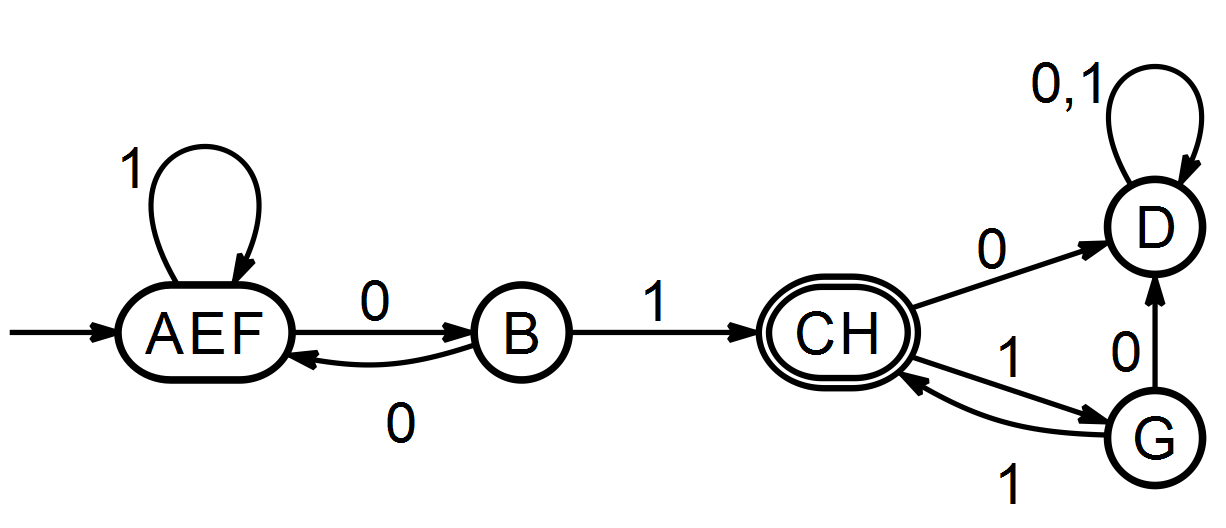
\includegraphics[width=\textwidth]{pics/det.png}  
  \end{center}
\end{frame}

\begin{frame}[fragile]
  \transwipe[direction=90]
  \frametitle{В предыдущей серии: распознание слова ДКА}
  \begin{center}
  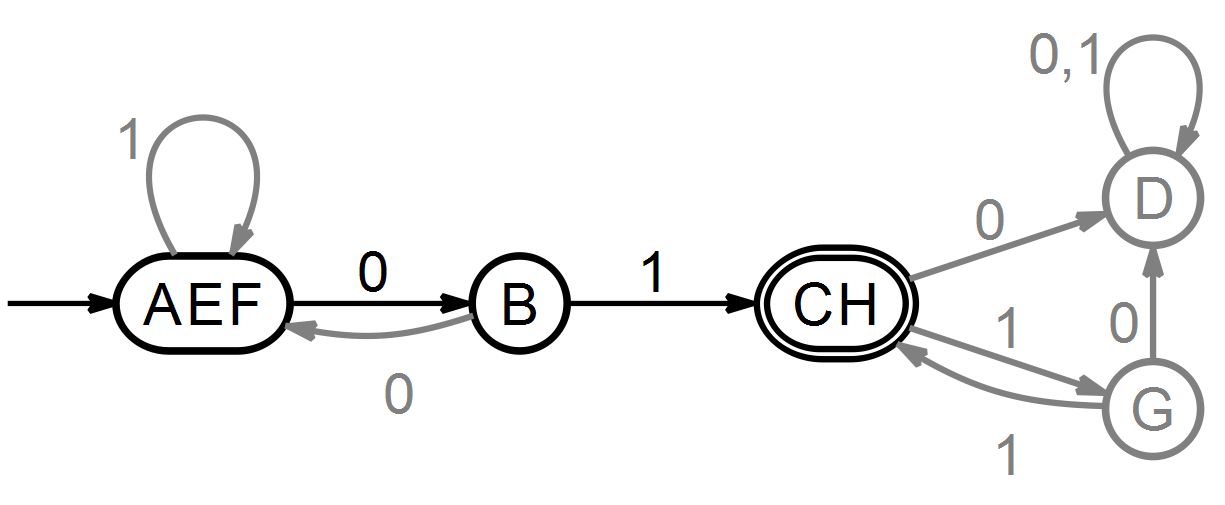
\includegraphics[width=\textwidth]{pics/path1.png}  
  \end{center}
\end{frame}

\begin{frame}[fragile]
  \transwipe[direction=90]
  \frametitle{В предыдущей серии: распознание слова ДКА}
  \begin{center}
  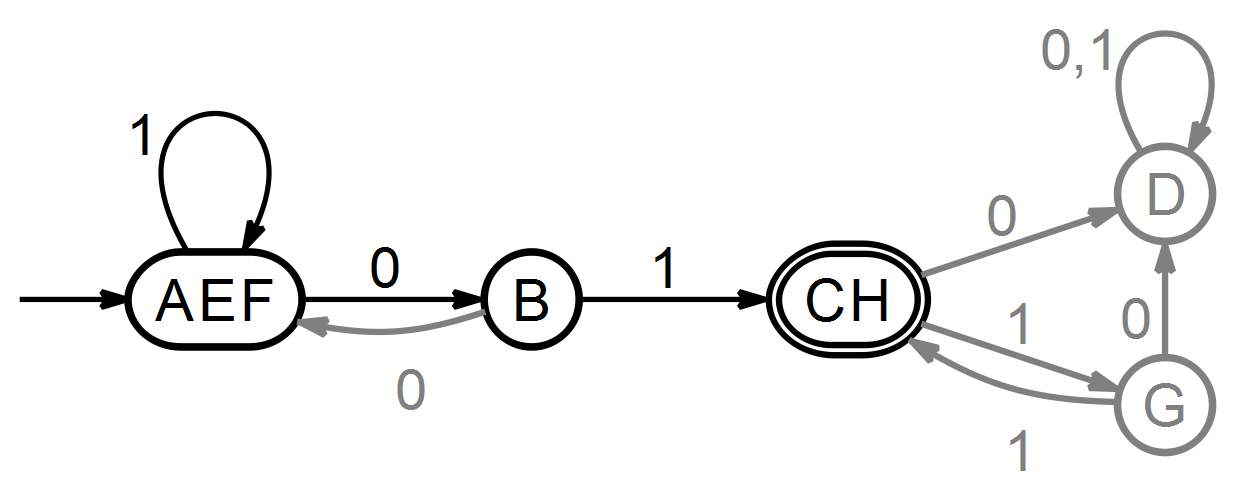
\includegraphics[width=\textwidth]{pics/path2.png}  
  \end{center}
\end{frame}

\begin{frame}[fragile]
  \transwipe[direction=90]
  \frametitle{В предыдущей серии: распознание слова ДКА}
  \begin{center}
  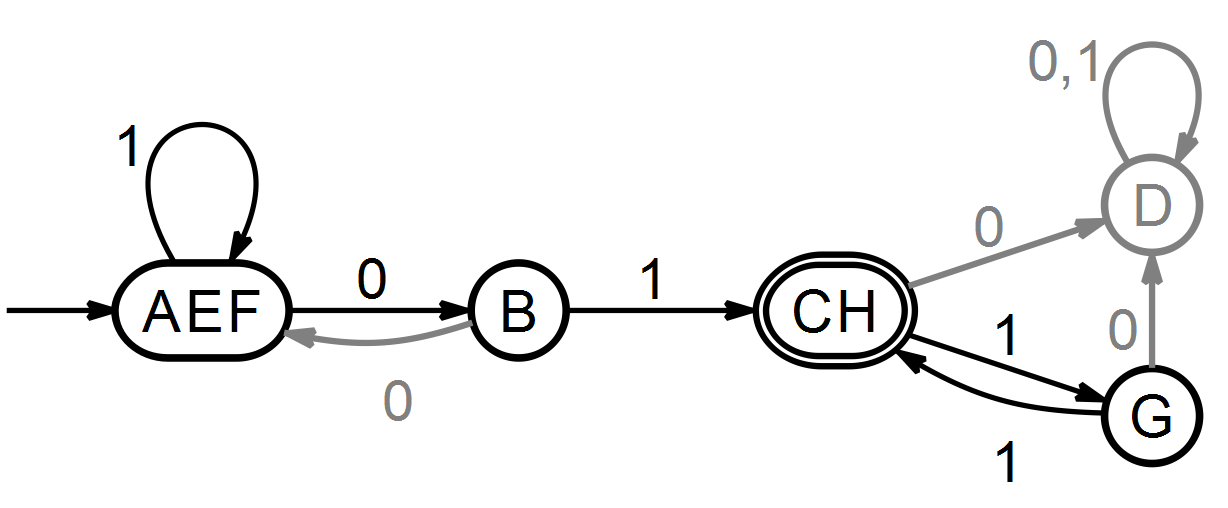
\includegraphics[width=\textwidth]{pics/path3.png}  
  \end{center}

  Слово распознается за $O(n)$
\end{frame}

\begin{frame}[fragile]
  \transwipe[direction=90]
  \frametitle{В предыдущей серии: распознание слова НКА}
  \begin{center}
  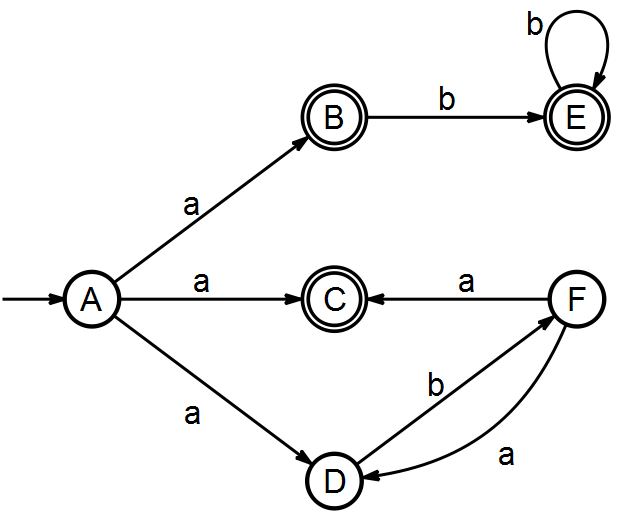
\includegraphics[height=0.75\textheight]{pics/2exdet.png}  
  \end{center}

  Слово распознается за $\dots$
\end{frame}

\begin{frame}[fragile]
  \transwipe[direction=90]
  \frametitle{В предыдущей серии: детерминизация}
  \begin{center}
  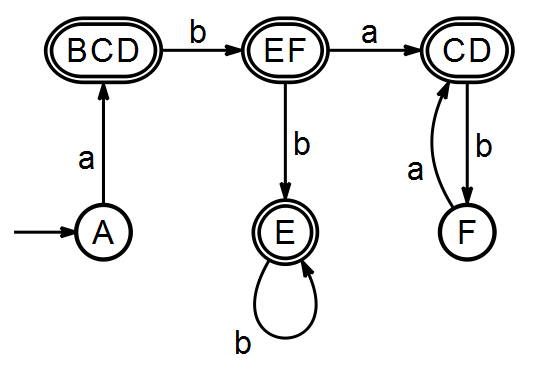
\includegraphics[height=0.75\textheight]{pics/2exdetres.png}  
  \end{center}

\end{frame}

\begin{frame}[fragile]
  \transwipe[direction=90]
  \frametitle{В предыдущей серии: минимизация}
  \begin{center}
  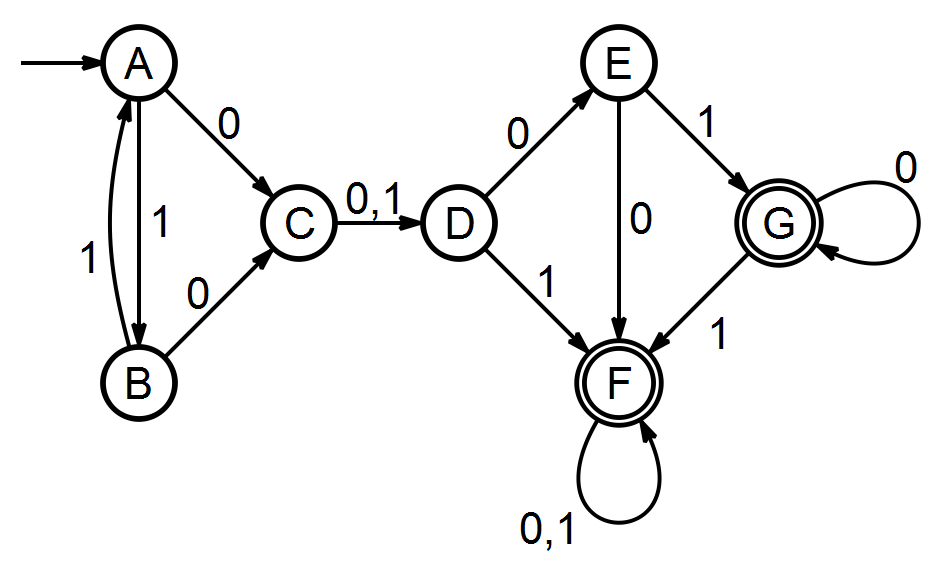
\includegraphics[width=0.5\textwidth]{pics/2exmin.png}  

  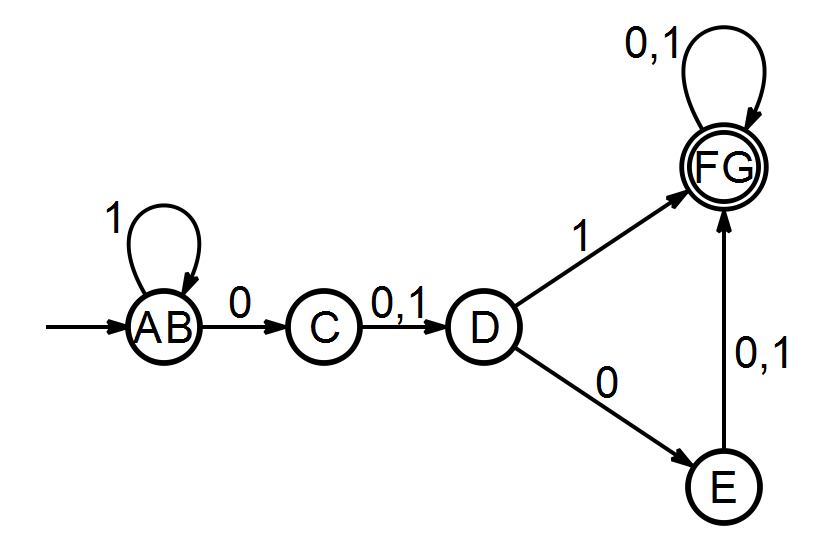
\includegraphics[width=0.5\textwidth]{pics/2exminres.png}  
  \end{center}

\end{frame}

\begin{frame}[fragile]
  \transwipe[direction=90]
  \frametitle{Произведение автоматов}
   $A_1 = \langle \Sigma_1, Q_1, q_{1_0}, \delta_1, F_1 \rangle$ и $A_2 = \langle \Sigma_2, Q_2, q_{2_0}, \delta_2, F_2 \rangle$ --- КА
  
  \textbf{Произведением} автоматов назовем $A = \langle \Sigma, Q, q_0, \delta, F \rangle$, где
  \begin{itemize}
    \item $\Sigma = \Sigma_1 \cup \Sigma_2$
    \item $Q = Q_1 \times Q_2$
    \item $q_0 = (q_{1_0}, q_{2_0})$
    \item $F \subseteq Q$
    \begin{itemize}
      \item $F = F_1 \times F_2$ --- распознает \textbf{произведение} языков
      \item $F = (F_1 \times Q_2) \cup (Q_1 \times F_2)$ --- распознает \textbf{объединение} языков
      \item $F = F_1 \times (Q_2 \setminus F_2)$ --- распознает \textbf{разность} языков
    \end{itemize}
    \item $\delta((q_1, q_2), c) = (\delta_1(q_1, c), \delta_2(q_2, c))$
  \end{itemize}
  
  Интуиция: ищем пути в двух автоматах одновременно
\end{frame}


\begin{frame}[fragile]
  \transwipe[direction=90]
  \frametitle{Произведение автоматов: пример}
  \begin{center}
  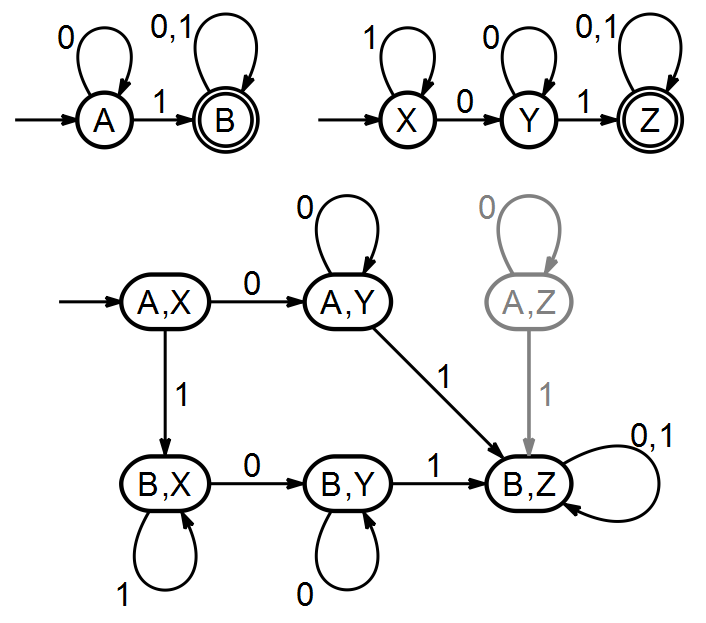
\includegraphics[width=0.7\textwidth]{pics/prod.png}  
  \end{center}
\end{frame}

\begin{frame}[fragile]
  \transwipe[direction=90]
  \frametitle{Пересечение языков}
  \begin{center}
  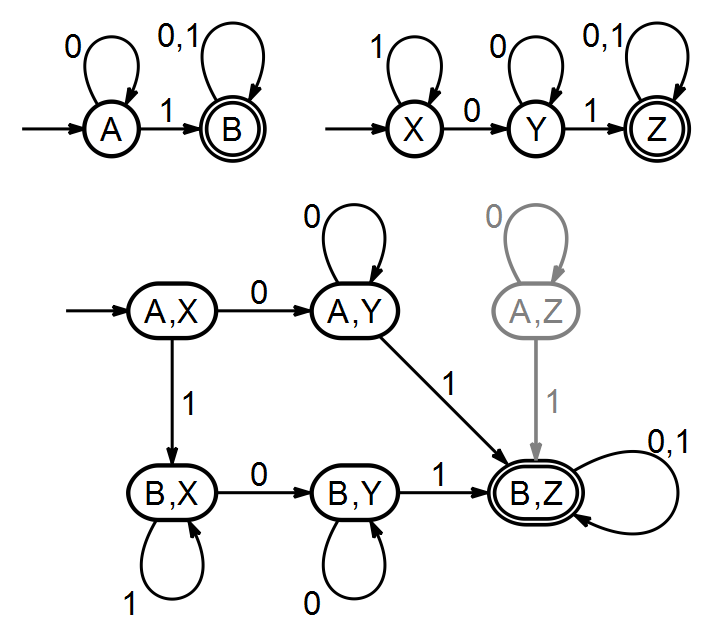
\includegraphics[width=0.7\textwidth]{pics/cap.png}  
  \end{center}
\end{frame}

\begin{frame}[fragile]
  \transwipe[direction=90]
  \frametitle{Объединение языков}
  \begin{center}
  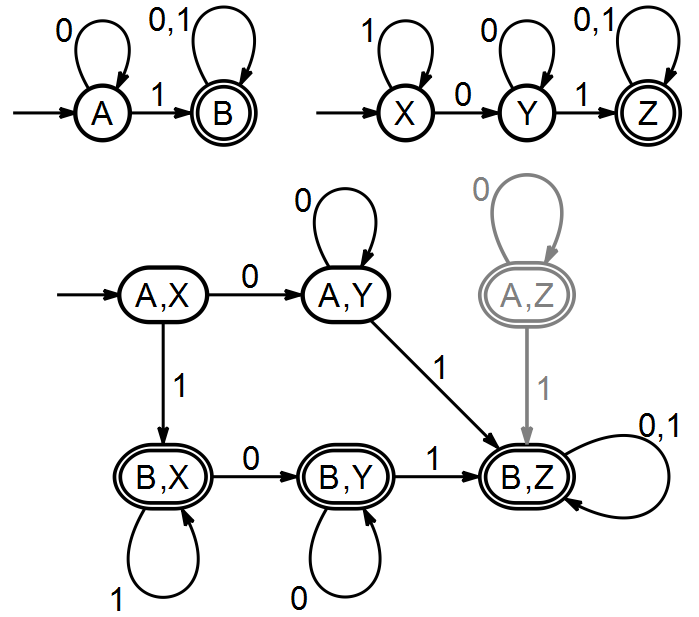
\includegraphics[width=0.7\textwidth]{pics/cup.png}  
  \end{center}
\end{frame}

\begin{frame}[fragile]
  \transwipe[direction=90]
  \frametitle{Разность языков}
  \begin{center}
  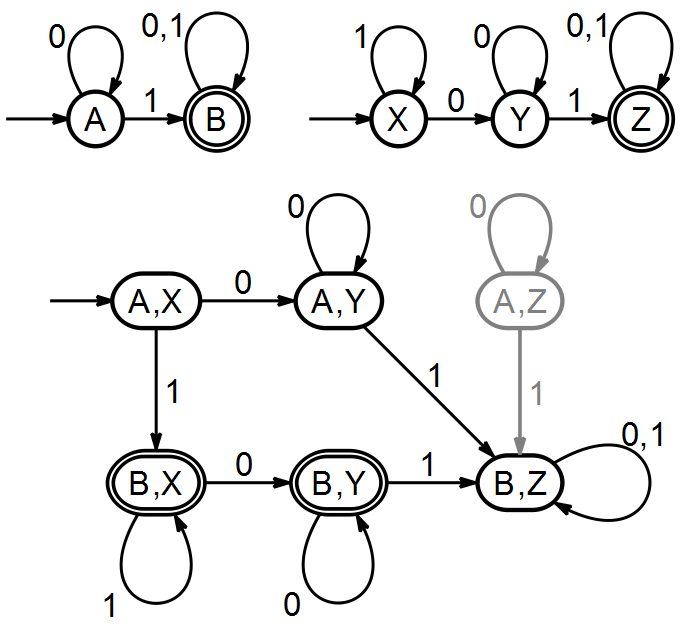
\includegraphics[width=0.7\textwidth]{pics/diff.png}  
  \end{center}
\end{frame}

\begin{frame}[fragile]
  \transwipe[direction=90]
  \frametitle{Замкнутость автоматных языков относительно операций}
  Автоматные языки замкнуты относительно операций 
  \begin{itemize}
    \item Объединения
    \item Пересечения
    \item Разности
    \item Дополнения
  \end{itemize}
\end{frame}

\begin{frame}[fragile]
  \transwipe[direction=90]
  \frametitle{Регулярное множество (регулярный язык)}
    \textbf{Регулярное множество} в алфавите $\Sigma$ определяется итеративно:
    \begin{itemize}
      \item $\varnothing $ --- регулярное множество в алфавите $\Sigma$
      \item $\{a\}$  --- регулярное множество в алфавите $\Sigma$ для каждого $a \in \Sigma$
      \item $\{\varepsilon\}$  --- регулярное множество в алфавите $\Sigma$
      \item Если $P$ и $Q$ --- регулярные множества в алфавите $\Sigma$, то регулярны
      \begin{itemize}
        \item $P \cup Q$ (объединение)
        \item $PQ$ (конкатенация, $\{ pq | p \in P, q \in Q\}$)
        \item $P^*$ (итерация: $P^* = \{\varepsilon\} \cup P \cup PP \cup PPP \cup \dots $)
      \end{itemize}
      \item Ничто другое не является регулярным множеством в алфавите $\Sigma$
      \item Множество всех регулярных языков обозначим $\mathbb{R}$
    \end{itemize}
\end{frame}

\begin{frame}[fragile]
  \transwipe[direction=90]
  \frametitle{Примеры регулярных языков}
  \begin{itemize}
   \item Все конечные языки
    \begin{itemize}
     \item $\{-2 147 483 648, -2 147 483 647, \dots,  2 147 483 647\}$ --- все 32-разрядные целые числа
    \end{itemize}
    \item $L_a = \{a^k \, | \, k - odd \} $
    \item $L_b = \{b^l \, | \, l - even \} $
    \item $L_{ab} = \{a^k b^l \, | \, k - odd, l - even\} =  L_a L_b$   
    \item $L = \{a^*\} = L_a^*$
  \end{itemize}
  
  
\end{frame}

\begin{frame}[fragile]
  \transwipe[direction=90]
  \frametitle{Регулярное выражение}
    \textbf{Регулярное выражение} --- способ записи регулярного множества
    \begin{itemize}
      \item $\varnothing $ --- обозначает $\varnothing$
      \item $a$  --- обозначает $\{a\}$ 
      \item $\varepsilon$  --- обозначает $\{\varepsilon\}$ 
      \item Если $p$ и $q$ обозначают $P$ и $Q$, то:
      \begin{itemize}
        \item $p | q$ обозначает $P \cup Q$ 
        \item $pq$ обозначает $PQ$
        \item $p^*$ обозначает $P^*$
      \end{itemize}
    \end{itemize}
\end{frame}

\begin{frame}[fragile]
  \transwipe[direction=90]
  \frametitle{Примеры регулярных выражений}
  \begin{itemize}
    \item $-2 147 483 648 | -2 147 483 647 | \dots |  2 147 483 647$ --- все 32-разрядные целые числа
    \item $a(aa)^*: L_a = \{a^k \, | \, k - odd \} $
    \item $(bb)^*: L_b = \{b^l \, | \, l - even \} $
    \item $a(aa)^* (bb)^* :  L_{ab} = \{a^k b^l \, | \, k - odd, l - even\} =  L_a L_b$   
    \item $a^* : L = \{a^*\} = L_a^*$
  \end{itemize}
\end{frame}


\begin{frame}[fragile]
  \transwipe[direction=90]
  \frametitle{Замкнутость регулярных языков относительно операций}
  Регулярные языки замкнуты ($A \in \mathbb{R}, B \in \mathbb{R} \Rightarrow A \diamond B \in \mathbb{R}$) относительно операций: 
  \begin{itemize}
    \item Конкатенации $ (L_1 L_2) $, объединения $ (L_1 \cup L_2) $, итерации $ (L^*) $
    \item Пересечения $ (L_1 \cap L_2) $, дополнения $ (\neg L)$, разности $ (L_1 \setminus L_2) $
    \item Обращения $(L_{rev} = \{a_m, a_{m-1}, \dots a_1 \, | \, a_1, a_2, \dots, a_m \in L \})$
    \item Гомоморфизма цепочек (операция сохраняющая $\varepsilon$ и конкатенацию)
    \item Обратного гомоморфизма цепочек
  \end{itemize}
\end{frame}


\begin{frame}[fragile]
  \transwipe[direction=90]
  \frametitle{Теорема Клини}
  \begin{rutheorem}
   Классы автоматных и регулярных языков \emph{эквивалентны}
  \end{rutheorem}
\end{frame}


\begin{frame}[fragile]
  \transwipe[direction=90]
  \frametitle{НКА с $\varepsilon$-переходами: почему бы и нет?}
  $\delta: Q \times (\Sigma \cup \varepsilon) \rightarrow 2^Q$
  
  \begin{center}
    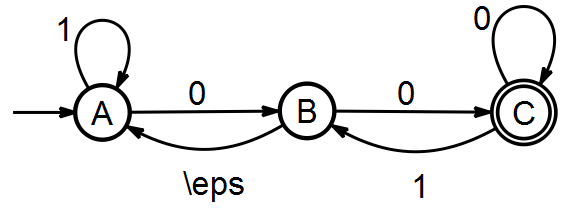
\includegraphics[width=0.75\textwidth]{pics/eps.png}  
  \end{center}
  
  Ничего не поломалось?
\end{frame}

\begin{frame}[fragile]
  \transwipe[direction=90]
  \frametitle{Эквивалентность НКА с $\varepsilon$-переходами и НКА без $\varepsilon$-переходов }
  \begin{itemize}
    \item НКА без $\varepsilon$-переходов --- частный случай НКА с $\varepsilon$-переходами
    \item В обратную сторону --- можно построить $\varepsilon$-замыкание
    \begin{itemize}
      \item Транзитивное замыкание: для каждого подграфа, состоящего только из $\varepsilon$-переходов, делаем $\varepsilon$-замыкание
      \item Добавление терминальных состояний: для $\varepsilon$-перехода из состояния $u$ в $v$, где $v$ --- терминальное, добавляем $u$ в терминальные
      \item Добавление ребер: $\forall u, v, c, w. \delta(u,\varepsilon)=v, \delta(v,c)=w$, добавим переход $\delta(u,c)=w$
      \item Устранение $\varepsilon$-переходов
    \end{itemize}
  \end{itemize}
\end{frame}

\begin{frame}
  \transwipe[direction=90]
  \frametitle{$\varepsilon$-замыкание}
  \begin{center}
    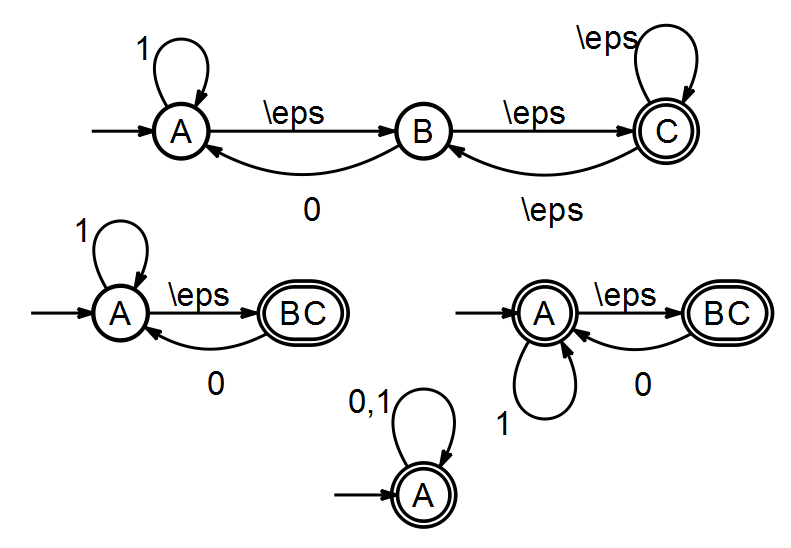
\includegraphics[width=0.85\textwidth]{pics/epsclosure.png}  
  \end{center}
 \end{frame}
 
\begin{frame}
  \transwipe[direction=90]
  \frametitle{Теорема Клини: доказательство $\Leftarrow$}
  
  \begin{rutheorem}
   Классы автоматных и регулярных языков \emph{эквивалентны}
  \end{rutheorem}
  
  \begin{proof}
    $\Leftarrow:$ Построим по регулярному выражению КА (НКА с $\varepsilon$-переходами)
  \end{proof}
\end{frame}

\begin{frame}
  \transwipe[direction=90]
  \frametitle{Построение КА по РВ: $\varepsilon$}
    \begin{center}
      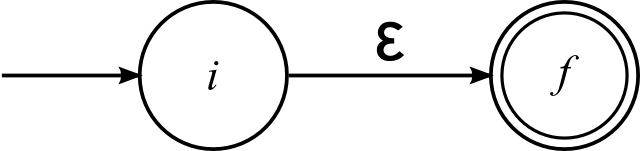
\includegraphics[width=0.40\textwidth]{pics/epsilon.png}  
    \end{center}
\end{frame}

\begin{frame}
  \transwipe[direction=90]
  \frametitle{Построение КА по РВ: символ}
    \begin{center}
      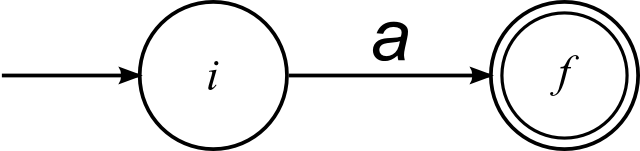
\includegraphics[width=0.40\textwidth]{pics/terminal.png}  
    \end{center}
\end{frame}

\begin{frame}
  \transwipe[direction=90]
  \frametitle{Построение КА по РВ: объединение $p | q$}
    \begin{center}
      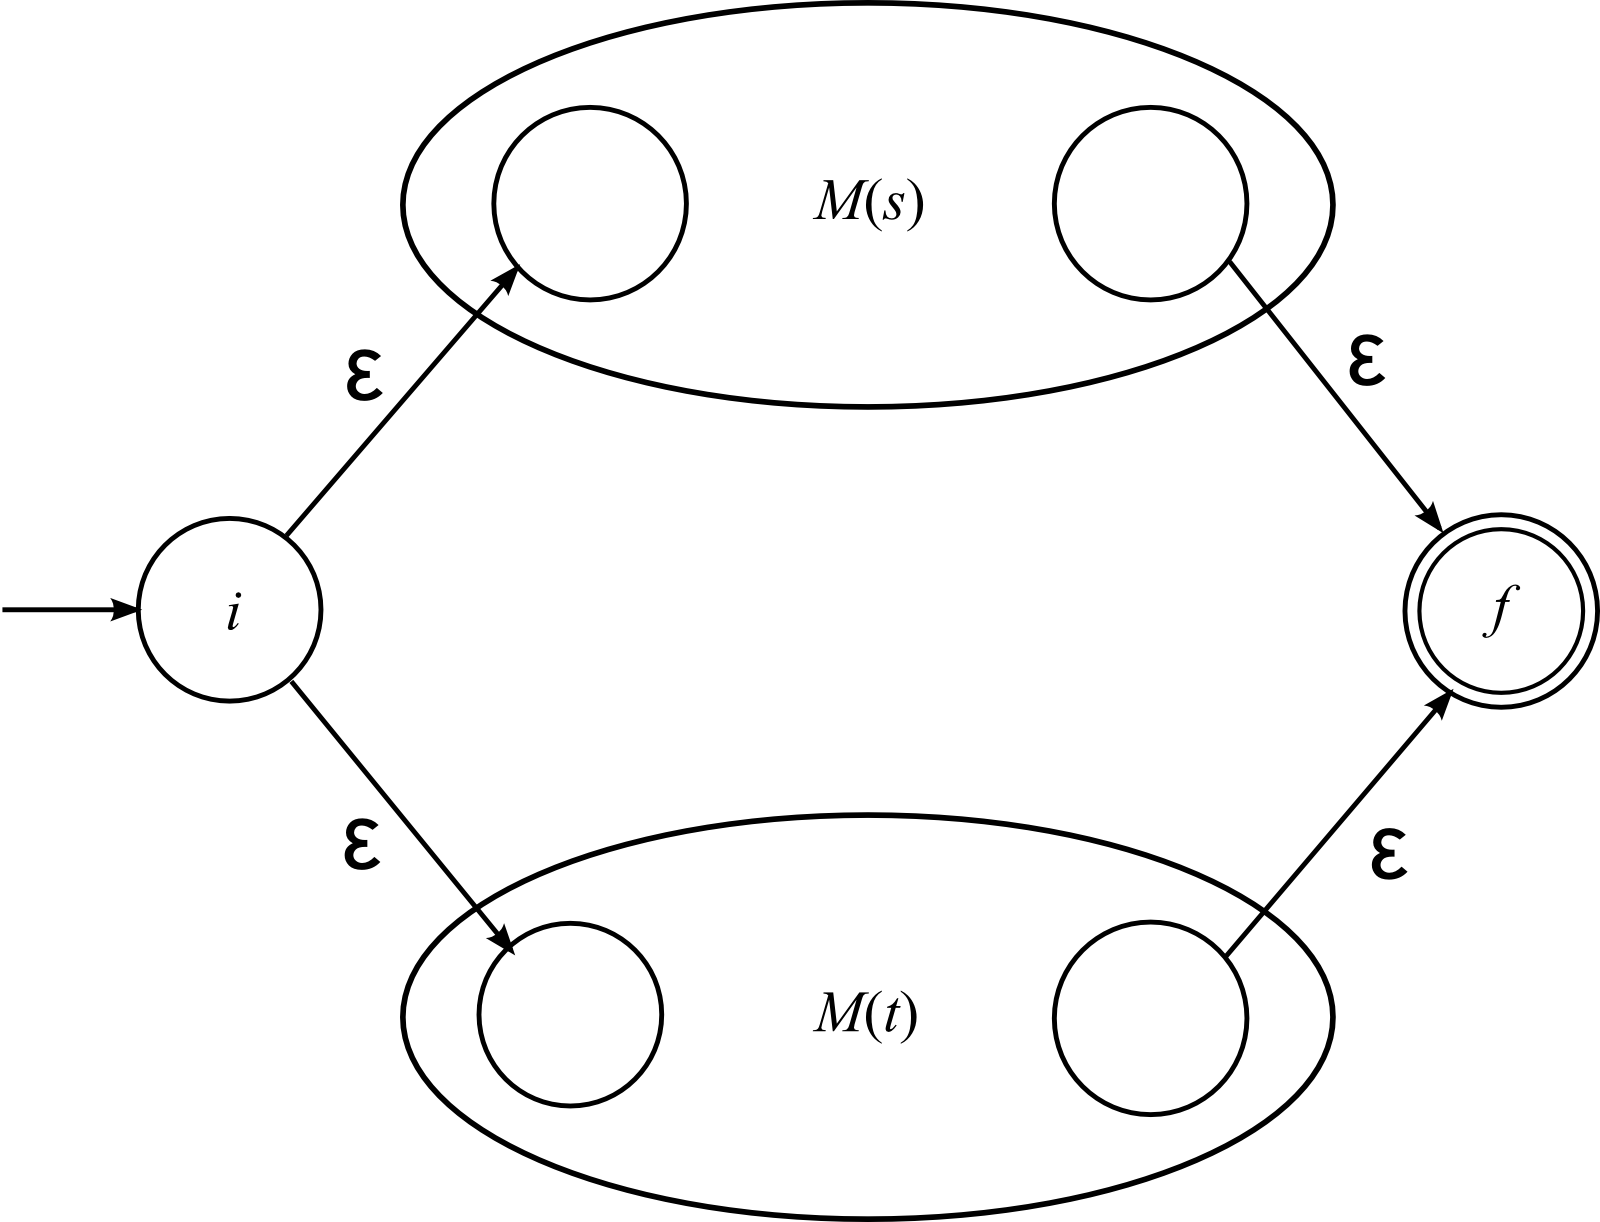
\includegraphics[width=0.80\textwidth]{pics/union.png}  
    \end{center}
\end{frame}

\begin{frame}
  \transwipe[direction=90]
  \frametitle{Построение КА по РВ: конкатенация $p q$}
    \begin{center}
      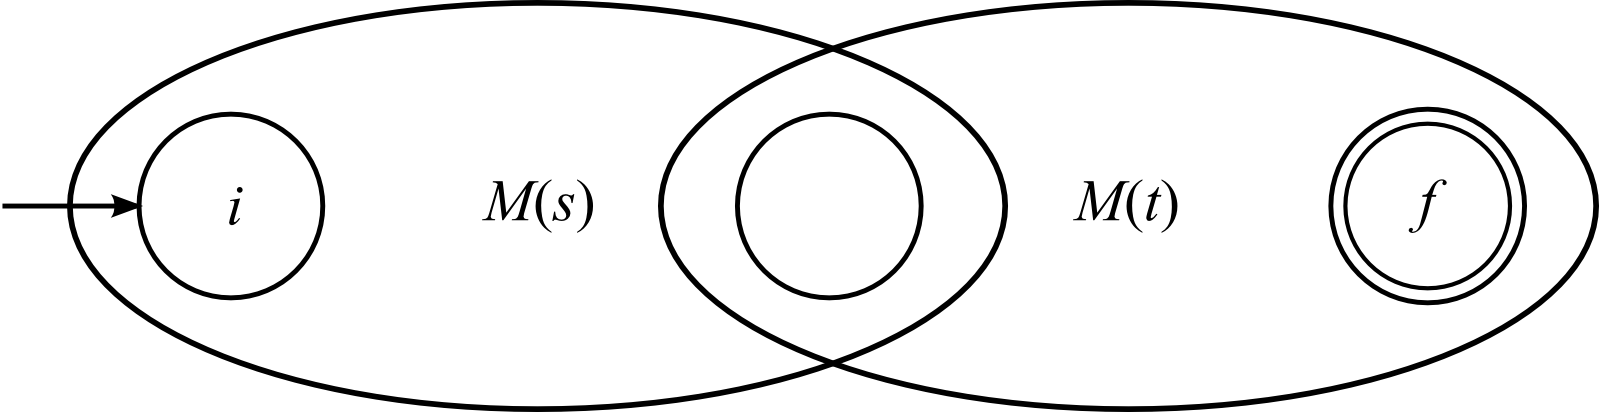
\includegraphics[width=0.80\textwidth]{pics/concat.png}  
    \end{center}
\end{frame}

\begin{frame}
  \transwipe[direction=90]
  \frametitle{Построение КА по РВ: итерация $p^*$}
    \begin{center}
      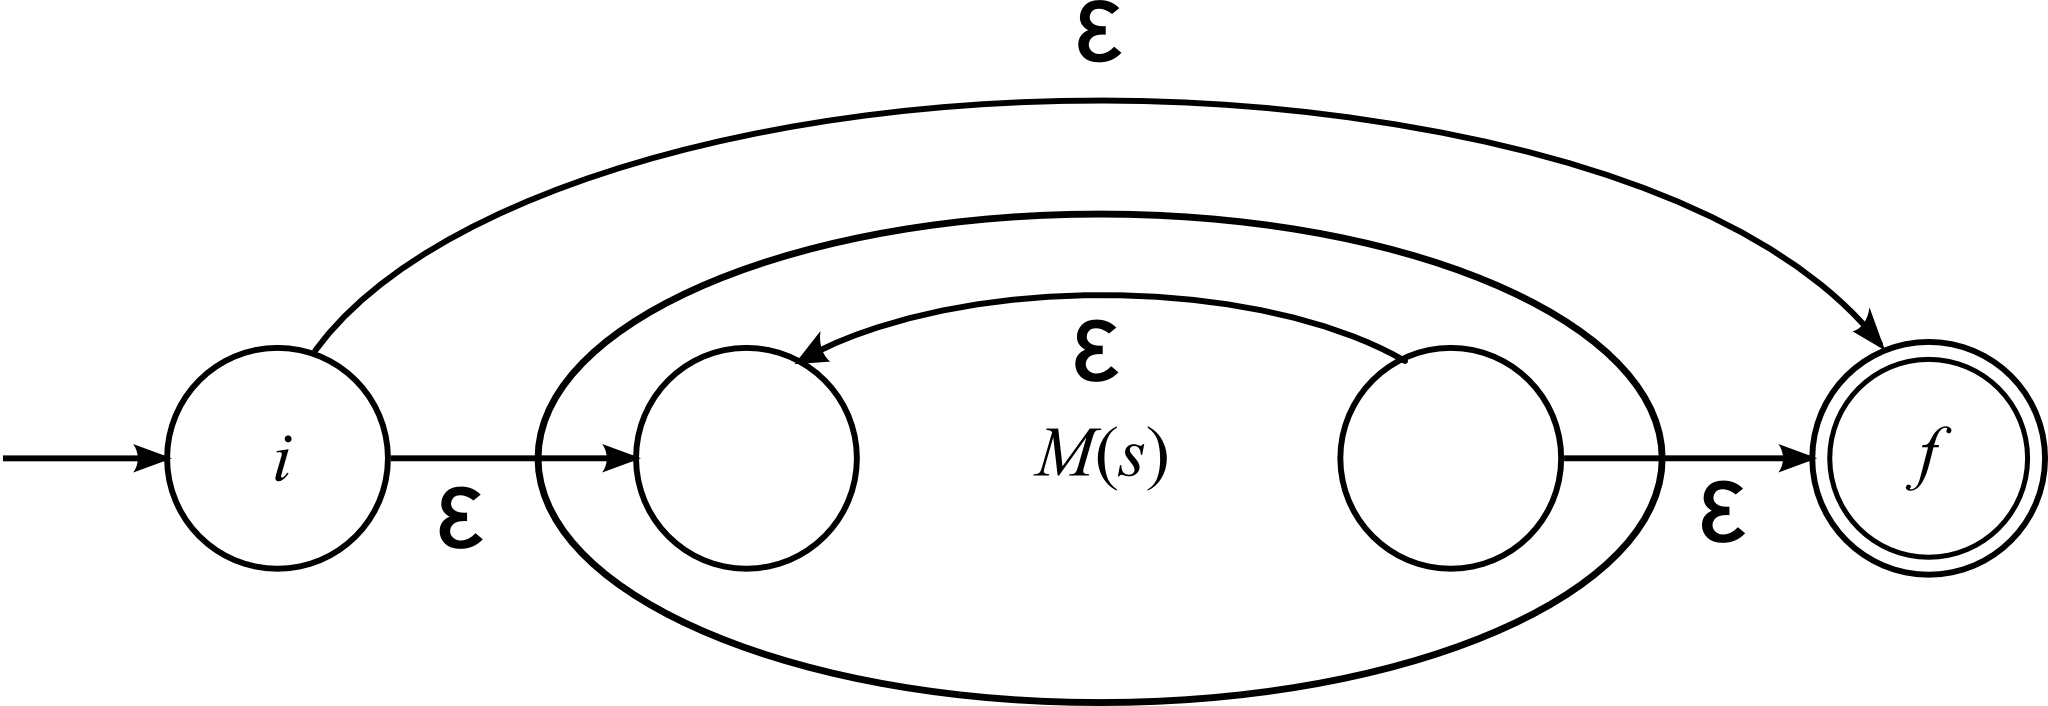
\includegraphics[width=0.80\textwidth]{pics/star.png}  
    \end{center}
\end{frame}

\begin{frame}
  \transwipe[direction=90]
  \frametitle{Теорема Клини: доказательство $\Rightarrow$}
  
  \begin{rutheorem}
   Классы автоматных и регулярных языков \emph{эквивалентны}
  \end{rutheorem}
  
  \begin{proof} 
   $\Rightarrow: $
    Построим регулярное выражение по конечному автомату методом исключения состояний
    
    Идея: на ребрах пишем регулярные выражения, соответсвующие путям между вершинами, последовательно исключаем состояния   
    
  \end{proof}
\end{frame}

\begin{frame}
  \transwipe[direction=90]
  \frametitle{Исключение состояния $s$}
    \begin{center}
      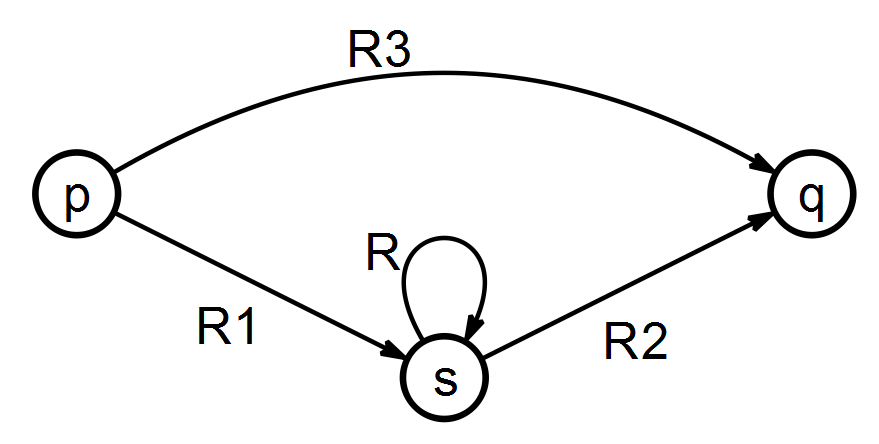
\includegraphics[width=0.60\textwidth]{pics/elim.png}  
      
      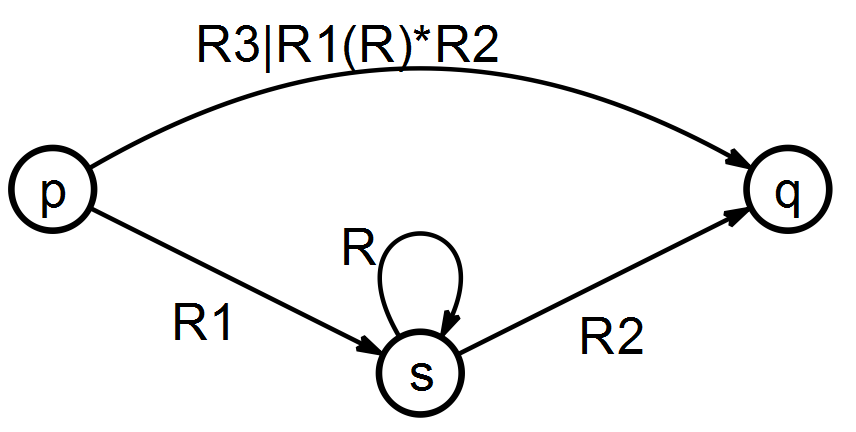
\includegraphics[width=0.60\textwidth]{pics/elim2.png}  
    \end{center}
\end{frame}

\begin{frame}
  \transwipe[direction=90]
  \frametitle{Исключение состояния $s$: удаление ребер и вершины}
    \begin{center}
      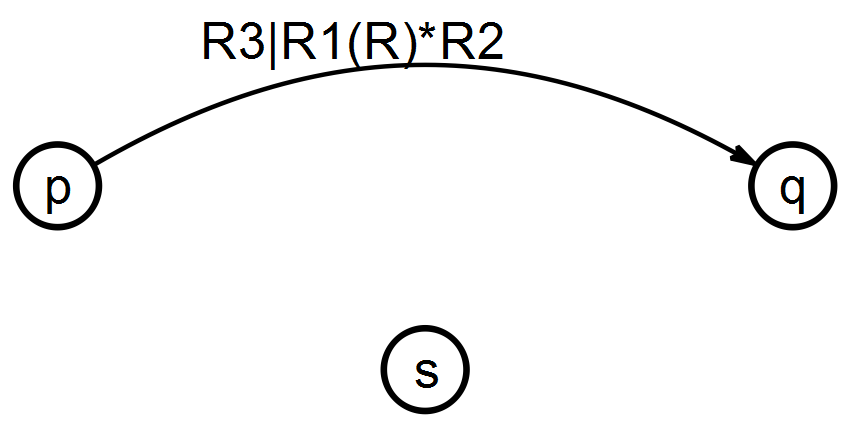
\includegraphics[width=0.60\textwidth]{pics/elim3.png}  
      
      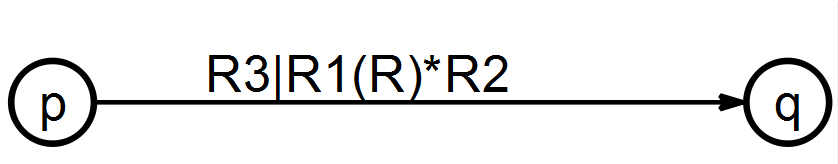
\includegraphics[width=0.60\textwidth]{pics/elim4.png}  
    \end{center}
\end{frame}

\begin{frame}
  \transwipe[direction=90]
  \frametitle{Исключение состояний: последний шаг}
    \begin{center}
      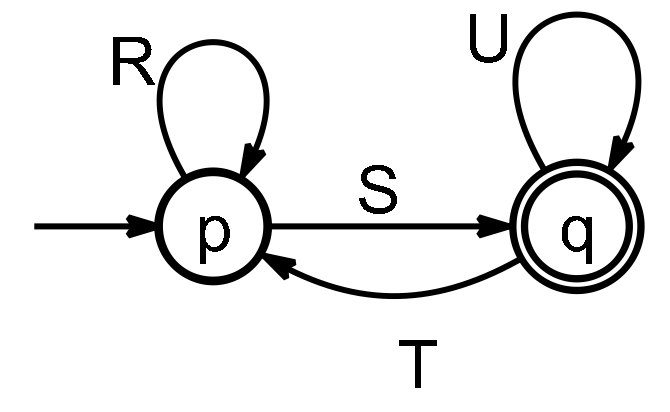
\includegraphics[width=0.6\textwidth]{pics/elim_final.png} 
    \end{center}

    $(R^* | S U^* T)^* S U^*$
\end{frame}

\begin{frame}
  \transwipe[direction=90]
  \frametitle{Исключение состояний: последний шаг}
    \begin{center}
      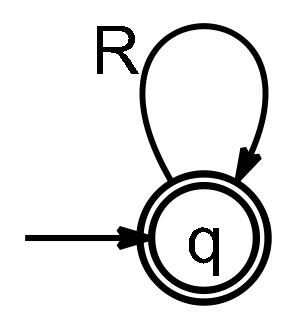
\includegraphics[width=0.3\textwidth]{pics/elim_final2.png}  
    \end{center}
    
    $R^*$
\end{frame}

\begin{frame}
  \transwipe[direction=90]
  \frametitle{Исключение состояний: пример}
    \begin{center}
      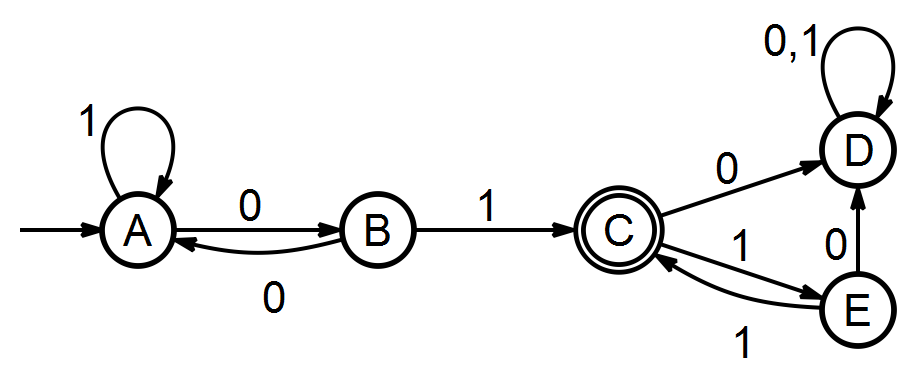
\includegraphics[width=0.60\textwidth]{pics/elim_ex.png}  
      
      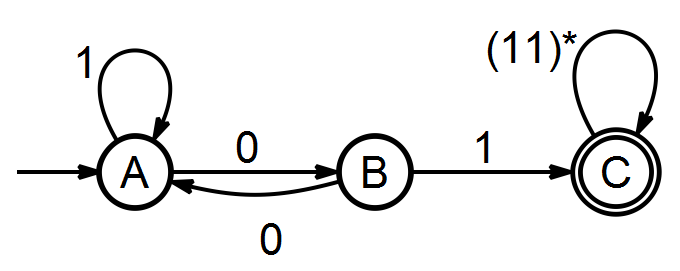
\includegraphics[width=0.45\textwidth]{pics/elim_ex2.png}  
            
      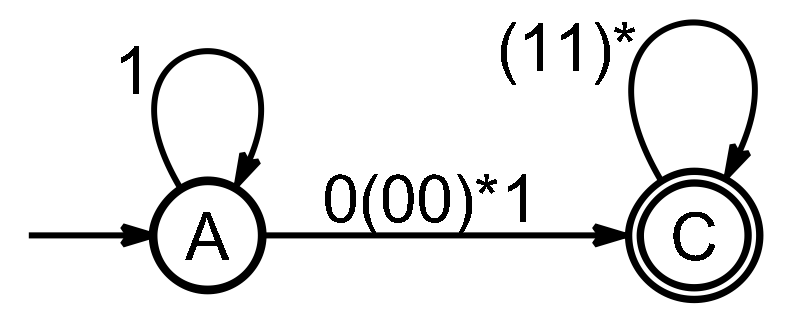
\includegraphics[width=0.35\textwidth]{pics/elim_ex3.png}  
    \end{center}
    
    $1^* 0 (00)^* 1 (11)^*$
\end{frame}

\begin{frame}
  \transwipe[direction=90]
  \frametitle{Свойства регулярных выражений}
  \begin{itemize}
    \item $a | a = a$
    \item $a | \varnothing = a$
    \item $a | b = b | a$
    \item $a | (b | c) = (a | b) | c$
    \item $a(bc) = (ab)c$
    \item $\{\varepsilon \} a = a \{ \varepsilon \} = \{ \varepsilon \} $
    \item $\varnothing a = a \varnothing = \varnothing$
    \item $a (b| c) = ab | ac$
    \item $(a | b) c = ac | bc $
    \item $\{\varepsilon \} | aa^* \subseteq a^*$
    \item $\{\varepsilon \} | a^*a \subseteq a^*$
    \item $ab \subseteq b \Rightarrow a^* b \subseteq b$
    \item $ab \subseteq a \Rightarrow a b^* \subseteq a$
        
  \end{itemize}
\end{frame}



\begin{frame}[fragile]
  \transwipe[direction=90]
  \frametitle{Регулярная грамматика}
  \textbf{Праволинейная грамматика} --- грамматика, все правила которой имеют следующий вид:
  \begin{itemize}
    \item $A \rightarrow a B$ или $A \rightarrow a$, где $A, B \in V_N, a \in V_T$
  \end{itemize}


  \textbf{Леволинейная грамматика} --- грамматика, все правила которой имеют следующий вид:
  \begin{itemize}
    \item $A \rightarrow B a$ или $A \rightarrow a$, где $A, B \in V_N, a \in V_T$
  \end{itemize}

\pause 

  \begin{rutheorem}[]
    Пусть L --- формальный язык. 

    $\exists G_r$ --- праволинейная грамматика, т.ч. $L = L(G_r) \Leftrightarrow \exists G_l$ --- леволинейная грамматика, т.ч. $ = L(G_l) $
  \end{rutheorem}
\pause
  \textbf{Регулярная грамматика} --- праволинейная или леволинейная грамматика
\end{frame}



\begin{frame}[fragile]
  \transwipe[direction=90]
  \frametitle{Эквивалентность регулярной грамматики и НКА}
  Алгоритм построения НКА $\langle Q, \Sigma, q_0, \delta, F \rangle$ по праволинейной грамматике $\langle V_T, V_N, P, S \rangle$
  \begin{itemize}
    \item $Q = V_N \cup \{q_f\}$
    \item $\forall (A \rightarrow a B) \in P. \delta (A, a) = B$
    \item $\forall (A \rightarrow a) \in P. \delta (A, a) = q_f$
    \item $q_0 = S$
    \item $\forall (B \rightarrow \varepsilon) \in P. B \in F$
  \end{itemize}
\end{frame}


\begin{frame}[fragile]
  \transwipe[direction=90]
  \frametitle{Пример построения НКА по регулярной грамматике}
  $S \rightarrow aS | aA | \varepsilon$
  
  $A \rightarrow b | bA$
  
  ~\\~
  \begin{center}
  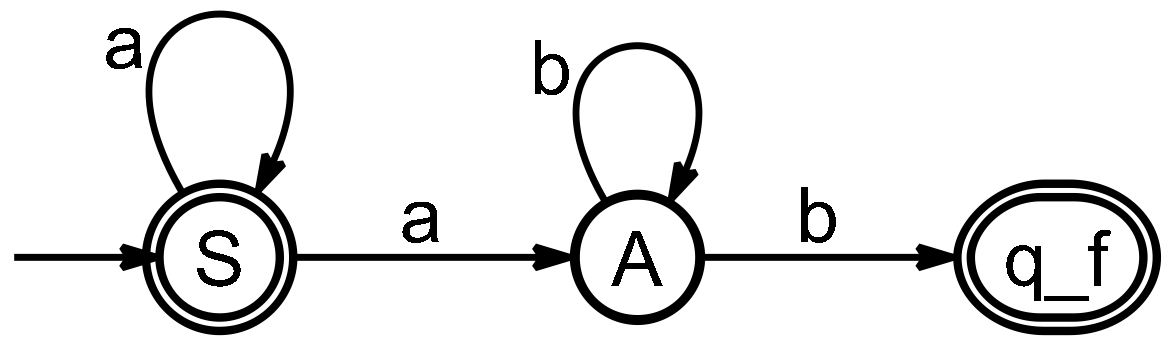
\includegraphics[width=0.60\textwidth]{pics/nfa_rg.png} 
  \end{center}
\end{frame}

\begin{frame}[fragile]
  \transwipe[direction=90]
  \frametitle{Эквивалентность регулярной грамматики и НКА}
  Алгоритм построения праволинейной грамматики $\langle V_T, V_N, P, S \rangle$ по НКА $\langle Q, \Sigma, q_0, \delta, F \rangle$
  \begin{itemize}
    \item $V_N = Q$
    \item $V_T = \Sigma$
    \item $\forall \delta(A, a) = B . (A \rightarrow a B) \in P$
    \item $\forall B \in F. (B \rightarrow \varepsilon) \in P$
    \item $S = q_0$
    \item Опционально: удалить $\varepsilon$-правила и бесполезные символы
  \end{itemize}
\end{frame}

\begin{frame}[fragile]
  \transwipe[direction=90]
  \frametitle{Пример построения НКА по регулярной грамматике}
  \begin{center}
  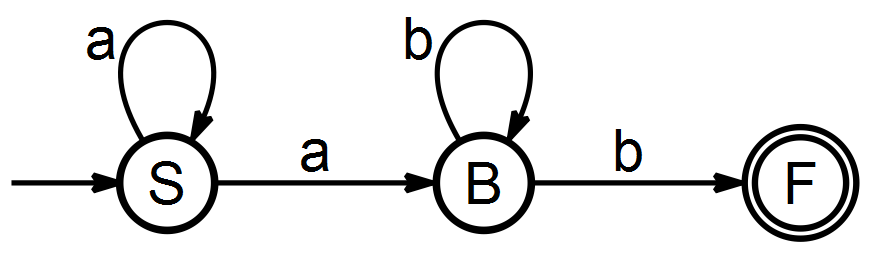
\includegraphics[width=0.60\textwidth]{pics/rg_nfa.png} 
  \end{center}
  
  ~\\~
  
   $S \rightarrow aS | aB$
  
  $B \rightarrow bB | aF$
  
  $F \rightarrow \varepsilon$
\end{frame}

\begin{frame}[fragile]
  \transwipe[direction=90]
  \frametitle{Пример построения НКА по регулярной грамматике}
  \begin{center}
  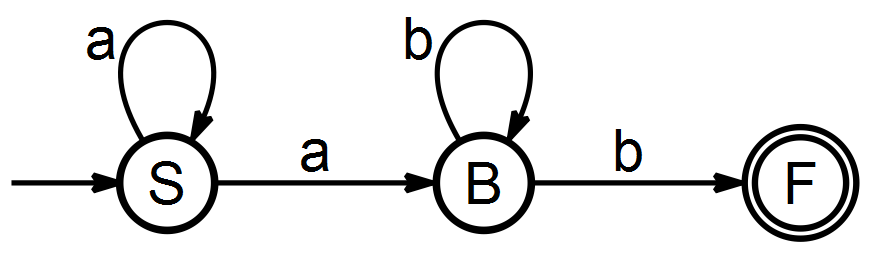
\includegraphics[width=0.60\textwidth]{pics/rg_nfa.png} 
  \end{center}
  
  ~\\~
  
   $S \rightarrow aS | aB$
  
  $B \rightarrow bB | a$
\end{frame}

\begin{frame}[fragile]
  \transwipe[direction=90]
  \frametitle{Лемма о разрастании (о накачке)}
  \begin{rutheorem}
  $L$ --- регулярный язык над $\Sigma \Rightarrow \exists n. \forall \omega \in L, | \omega | > n$
  
    $\exists x, y, z \in \Sigma^*. \, xyz = \omega, y \neq \varepsilon, |xy| \leq n,$
    
     $ \forall k \geq 0. \, x y^k z \in L$
  \end{rutheorem}
  
  \begin{proof}
  Строим автомат, распознающий $L$.
  
  Обозначаем за $n$ число состояний автомата.
  
  Слово длины большей, чем $n$, обязано при разборе пройти через одно состояние дважды --- получили цикл. 

  Метка цикла --- искомое $y$, по циклу можно пройти сколько угодно раз.
  
  \end{proof}

\end{frame}


\begin{frame}[fragile]
  \transwipe[direction=90]
  \frametitle{Использование леммы о накачке}
  \begin{itemize}
    \item $L = \{ (^k )^k | k \geq 0\} $
    \item Предполагаем, что $L$ --- регулярный язык
    \item Берем $n$ из леммы, рассматриваем слово $(^n )^n$
    \item Его можно разбить на $xyz, y \neq \varepsilon, |xy| \leq n$
    \item $|xy| \leq n \Rightarrow y = (^b, b > 0$
    \item Берем $k = 2$. $xy^kz = (^{n+b} )^n$, что не принадлежит $L$
    \item Получили противоречие $\Rightarrow L$  не регулярен
  \end{itemize}
  
\end{frame}


\begin{frame}[fragile]
  \transwipe[direction=90]
  \frametitle{Резюме}
  \begin{itemize}
    \item ДКА, НКА, НКА с $\varepsilon$-переходами, регулярные выражения, регулярные грамматики --- все эти формализмы задают один класс (регулярных) языков и эквивалентны друг другу
    \item Проверка принадлежности слова регулярному языку осуществляется за $O(n)$ и не требует дополнительной памяти
    \item Класс регулярных языков обладает хорошими свойствами, прост и нагляден
    \item С помощью леммы о накачке можно доказать нерегулярность языка
  \end{itemize}
  
\end{frame}


\end{document}
